
  
  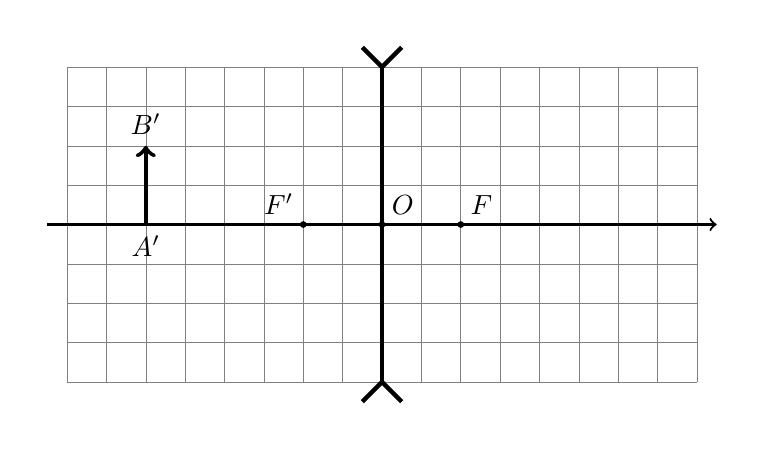
\begin{tikzpicture}[scale=0.5]
    \clip (-9,-5) rectangle (9,5) ;
    \draw [help lines] (-8,-4) grid [step=1] (8,4) ; %% Le quadrillage
    \draw [->,thick] (-8.5,0) -- (8.5,0) ; %% L'axe optique
    \draw [ultra thick] (0,-4) -- (0,4)  ; %% Le corps du systeme 

    % Dessin de la lentille et des points focaux
    \draw [ultra thick] (-0.5,-4.5) -- (0,-4) -- (0.5,-4.5)
                         (-0.5,4.5) -- (0, 4) -- (0.5,4.5) ;
    \filldraw [black] (-2.0,0) circle (2pt) node [above left] {$F'$};
    \filldraw [black] (2.0,0) circle (2pt) node [above right] {$F$} ;
    \filldraw [black] (0,0) circle (2pt) node [above right] {$O$} ;
    
      \draw [->,ultra thick] (-6.0,0) node [below] {$A'$} -- (-6.0,2.0) node [above] {$B'$} ;
      
  \end{tikzpicture}
